\chapter{Conclusiones y trabajos futuros}
\title{Conclusiones y trabajos futuros}

\section{Pruebas realizadas}
\title{Pruebas realizadas}

En las figuras \ref{fig:protodirector} y \ref{fig:protomusico} se muestra cómo se han
implementado los dos dispositivos.

\begin{figure}[!htb]
\centering
\captionsetup{justification=centering}
\includegraphics[width=0.8\textwidth]{./imagenes/prototipodirector}
\caption{Prototipo del dispositivo director} \label{fig:protodirector}
\end{figure}

\begin{figure}[!htb]
\centering
\captionsetup{justification=centering}
\includegraphics[width=0.8\textwidth]{./imagenes/prototipomusico}
\caption{Prototipo del dispositivo músico} \label{fig:protomusico}
\end{figure}


\begin{figure}[htb]
\centering
\captionsetup{justification=centering}
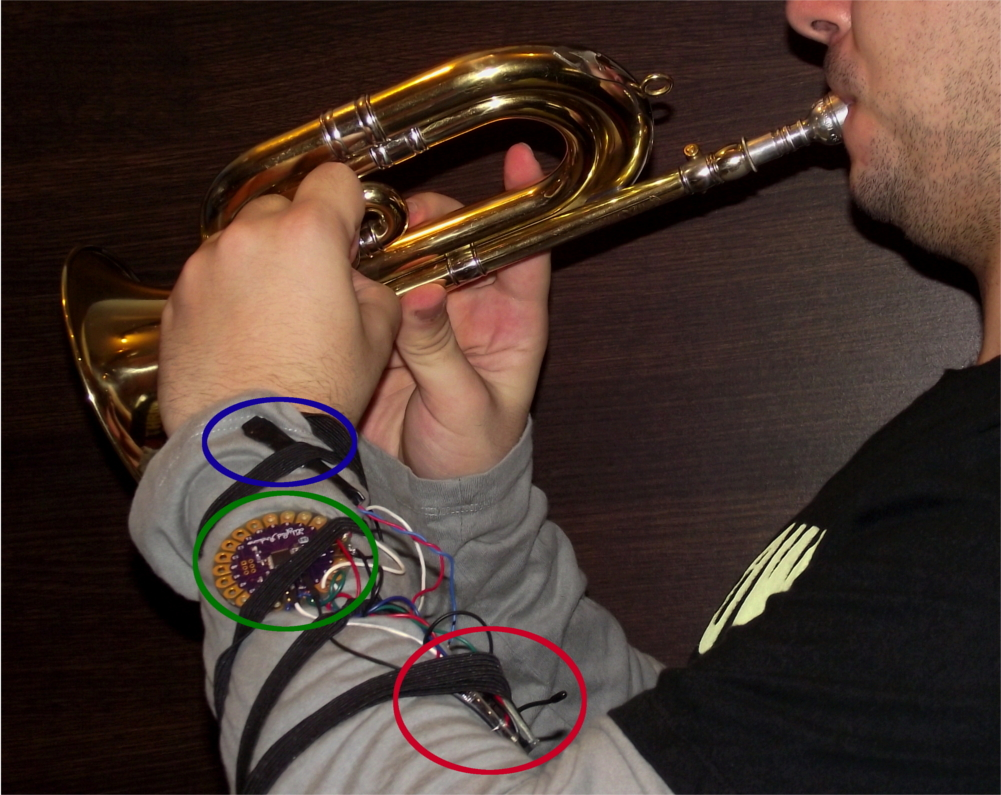
\includegraphics[width=0.8\textwidth]{./imagenes/musicoprobando}
\caption{Un músico probando el prototipo} \label{fig:musicoprobando}
\end{figure}

Para probar que el dispositivo satisface las necesidades de los usuarios, se ha
probado un prototipo durante un ensayo de la ``Asociación Musical Cultural La Victoria"
de Fuente Vaqueros (Granada). Aunque al principio la reacción por parte de los músicos
fue un poco reacia, al poner el sistema en funcionamiento, vieron en él una gran
oportunidad para mejorar la calidad musical del grupo.\\

En la figura \ref{fig:musicoprobando}, podemos ver un músico probando un prototipo
del sistema durante un ensayo (durante el experimento, se utilizaron gomas eslásticas para sujetar toda
la circuitería, permitiendo sujeción al aparato y la movilidad del músico).
\begin{itemize}
  \item \textcolor{blueS}{$\blacksquare$} Dispositivo actuador: es decir,
  el micromotor vibrador
  \item \textcolor{green}{$\blacksquare$} Controlador: Arduino Lilypad
  \item \textcolor{red}{$\blacksquare$} Mota: \textit{shield} con el XBee
\end{itemize}






\section{Comparación con otros dispositivos del mercado}
\title{Comparación con otros dispositivos del mercado}
Ya en la introducción de hablaba de Body Beat, de la marca Peterson \cite{bodybeat}.\\

\begin{description}
  \item[Funcionalidad] \hfill \\
    Body Beat dispone de una amplia gama de funciones como posibilidad de introducir
    obras en MIDI (un estándar que permite la interconexión de instrumentos musicales,
    ordenadores, tarjetas de sonido y otros dispositivos, pudiendo secuenciar las señales
    emitidas por todos ellos, volcarlo a un fichero y reproducirlo como sonido), utilización
    de un altavoz integrado... mientras que ArduBand solo permite, cuando este trabajo
    se está escribiendo, la sincronización entre músicos de una banda para mantener
    el mismo tempo aunque, a partir de la infraestructura con la que se cuenta, se pueden
    desarrollar muchas nuevas funcionalidades (como los que se verán en la sección ``Trabajos futuros")

  \item[Licencia de desarrollo] \hfill \\
    Body Beat es un dispositivo cerrado cuyo único desarrollador es Peterson (y aquellas otras
    compañías que se encuentren subcontratadas). ArduBand es un proyecto libre, lo que
    ayudará a aumentar el número de funcionalidades y subsanar los errores que puedan aparecer

  \item[Precio] \hfill \\
    El precio de BodyBeat es de unos 139.99USD (unos 126\euro). Para contar con el pack más básico de ArduBand, es
    necesario comprar un dispositivo músico y un dispositivo director. Si sumamos los costos
    calculados en \ref{table:costodirector} y \ref{table:costomusico}, el coste asciende a 97.5\euro.
    Ahora, si estimamos que en cada dispositivo tenemos 10\euro\ de beneficio (como ya se hizo en \ref{sec:ganancia},
    el precio asciende a 117.5\euro\ (el costo de fabricar los dispositivos y 10\euro\ de beneficio por uno). El precio
    es muy ajustado pero, teniendo en cuenta que a nuestro dispositivo hay que añadir los gastos de ingeniería (entre otros),
    ArduBand sale perdiendo. La ventaja de ArduBand frente a Body Beat, tiene lugar cuando
    se compran muchos dispositivos:\\
    Supongamos que disponemos de una banda de música con 100 músicos (entre ellos el director)
    y queremos implantar el sistema:\\
    \underline{Implantando Body Beat}
    \[
      100 \times 126 = 12.600 \textup{\euro}
    \]
    \underline{Implantando ArduBand}
    \[
      99 \times 46.5 + 51 = 5.654,5 \textup{\euro}
    \]
    La diferencia es considerable aunque esto es un cálculo orientativo ya que, como ya se ha mencionado,
    no se estarían ganando 10\euro\ por cada dispositivo (al tener que añadir otros gastos). También
    habría que añadir el precio de 100 batería externas (el modelo \textit{A5 Classic} de la marca \textit{Power Bank} se puede
    adquirir por 6\euro, lo que sumaría 600 \euro\ al precio final).\\
    Por otro lado, a Body Beat hay que añadirle un gran inconveniente: es difícil
    obtenerlo en España, por lo que se habría que encargarlo a EEUU, aumentando el costo
    debido al pago de servicios aduaneros y/o gastos de envío
  \item[Tamaño] \hfill \\
    Body Beat tiene un tamaño de 4.25" x 3" x 1" (10,795cm x 7,62 cm x 2,54 cm, aproximadamente).
    ArduBand se presenta en dos formatos (teniendo en cuenta las caracasas): director (5,8 cm de diámetro x 3,2cm de altura,
    aproximadamente) y músico (5,8 cm de diámetro y 2,3 de altura, aproximadamente). Si calculamos los tres volúmenes (para facilitar
    el cálculo, se toma que los dispositivos ArduBand son una aproximación a cilindo -aunque, realmente es algo menor-),
    Body Beat es de unos 209cm\textsuperscript{3}, el dispositivo director 84.5cm\textsuperscript{3} y el
    músico 60.8cm\textsuperscript{3}. Hay que añadir al volúmen de los dispositivos ArduBand, el de una batería externa. Por
    ejemplo, si adquirimos la que se ha mencionado anteriormente (el modelo \textit{A5 Classic} de \textit{Power Bank}), tenemos
    que añadir un volumen de 50cm\textsuperscript{3} (9,6cm x 2.4 cm x 2.2cm). Además de que el volumen sigue siendo menor
    al de Body Beat,  la posibilidad de guardar la batería en otro lugar (como un bolsillo), hace que sea menos vistoso.\\
    También el peso es menor en ArduBand (en ArduBand ronda los 150g y BodyBeat sobrepasa los 300g)
  \item[Batería] \hfill \\
    En Body Beat, la batería viene integrada y es de 500mA (aunque no se especifique, se entiende que son 500mAh). En ArduBand,
    es el usuario el que elige qué batería usar. Por ejemplo, podríamos volver a elegir el modelo \textit{A5 Classic}
    de \textit{Power Bank} (en cuyo caso, tendríamos disponibles 2.600mAh, el quíntuple de la que trae integrada Body
    Beat).\\
    Body Beat dispone de varios sensores/actuadores que consumen energía, mientras que en ArduBand, el número
    de dispositivos es muy reducido (por lo que habrá un menor consumo eléctrico y mayor duración
    de la batería)
  \item[Utilizar el \textit{watch dog} de Arduino] \hfill \\
    Es un mecanismo que reinicia un dispositivo en caso que se detecte que se ha producido un bloqueo.
    Un trabajo de futuro será utilizar este sistema para,
    en caso de error, que los dispositivos puedan recuperarse solos.
  \item[\textit{Hardware} propio] \hfill \\
    Para disminuir el tamaño de los dispositivos, queda como actividad para analizar en un futuro, la posibilidad
    de crear un \textit{hardware} propio, es decir, una placa integrada que llevase todos los componentes necesarios
    para hacer funcionar cada dispositivo.
  \item[Otros] \hfill \\
    En caso de ser necesario cambiar algún componente por que se haya estropeado, en Body Beat habría que enviarlo
    al servicio técnico. ArduBand, si consigue establecer una comunidad a su alrededor, un usuario podría reparar
    su propio dispositivo gracias a los desarrolladores. Además, si se quiere sustituir, por ejemplo, la batería,
    habría que comprarla a la empresa ``Peterson" (cuando se comparaba el precio, se comentaba el problema que hay
    para encontrar el dispositivo -y añadidos- en España).
\end{description}



\section{Trabajos futuros}
\title{Trabajos futuros}
Durante todo este trabajo se ha hecho hincapié en la posibilidad de aumentar la
funcionalidad del proyecto o, gracias al carácter que le otorga el ser libre,
que nazcan nuevas implementaciones del mismo sistema.\\

Algunos trabajos futuros propuestos son:
\begin{description}
    \item[Sincronización de partituras] \hfill \\
      Ya que se está sincronizando a los músicos, se podría aumentar el tamaño de la traza
      que se envía, permitiendo que cada músico sepa por dónde está interpretando la banda.
      Por sí solo ya sería útil pero, añadiendo una pantalla (de tinta electrónica, para que el consumo
      sea más bajo) o utilizando un dispositivo móvil (una \textit{tablet} o teléfono), las partituras
      podrían ``reproducirse" solas y a la vez (de similar forma a la que lo hacen softwares de edición
      de partituras como Encore -anteriormente de Gvox y ahora de Passport Music Software-, Sibelius -de Avid Technology-,
      Finale -MakeMusic- MuseScore -un proyecto libre de Werner Schweer-).\\
      Teniendo en cuenta la actual duración de las baterías, esto solo sería viable para ensayos.\\
      Dando un paso más, sería interesante introducir ``Google Cardboard" \cite{cardboard} (una estructura
      para utilizar el teléfono móvil como gafas de realidad aumentada/virtual que dispone de SDK propio, desarrollado por Google)
      en las bandas de música para visionado de partituras (de nuevo, solo para ensayo)

    \item[\textit{Feedback}] \hfill \\
      Utilizando distintos sensores, conocer cuánto falla la banda respecto al tempo marcado (y así estudiar
      puntos a mejorar en la interpretación). Por ejemplo, la colocación de un sensor de vibración
      en los parches inferiores de los intrumentos de percusión nos daría información sobre el tempo que están
      siguiendo estos instrumentos.\\
      Si, se consiguiera además, medir esta variable en cada músico, la aplicación de técnicas de gamificación
      sería un punto a tener en cuenta para motivar a los músicos a mejorar

    \item[Utilización de otras plataformas] \hfill \\
      Una vez superados los problemas vistos a lo largo de la memoria, estudiar cambiar algunas de las plataformas
      elegidas por otras que fueron desestimadas anteriormente, es un campo en el que trabajar para obtener mejores
      resultados. Por ejemplo, en vez de utilizar motas ZigBee, utilizar otras que usen 802.15.4 (para eliminar
      el retardo que se produce debido a que cada paquete tiene que pasar por las capas de 802.15.4 y por las de ZigBee).\\
      La utilización de motas para redes de sensores cuyos diseños tengan una licencia libre o utilicen sistemas
      operativos de código abierto (como TinyOS o Contiki) es algo que habrá que investigar, ya que se quieren
      utilizar plataformas abiertas para este desarrollo.

    \item[Creación de aplicaciones para más SO móviles] \hfill \\
      Ya que casi todos los dispositivos móviles disponen de Bluetooth, para llegar al mayor número de usuarios
      posible, sería útil el desarrollo de una aplicación para cada uno de los principales sistemas operativos
      móviles del mercado. Además, habrá que finalizar la implementación de la aplicación Android que se ha creado
      en este proyecto, utilizando la guía de estilos de Google.

     \item[Mejorar fiabilidad de la red y facilitar su uso] \hfill \\
      Que el usuario pueda añadir nuevos dispositivos de tipo músico de una forma sencilla, es uno de los
      trabajos que habrá que tener en cuenta para futuras versiones del proyecto. Por supuesto
      también sería interesante mejorar la fiabilidad de la red, pudiendo añadir múltiples directores
      (y que manden en la red según algún sistema de prioridades) por si hay problemas con el
      dispositivo director principal

\end{description}

\subsection{Posibilidades en el futuro}
\title{Posibilidades en el futuro}
En cuanto al futuro de las tecnologías utilizadas, ya se pudo ver las previsiones
de la curva de Gartner (figura \ref{fig:curvaG} y \cite{gartnercurve}) que, tanto dispositivos \textit{wearables} como
aquellos relacionados con el ``Internet de las cosas"\ (como las redes de sensores), tendrán un gran protagonismo
en nuestra vida. Como consecuencia de ello, los distintos elementos para fabricarlos
verán reducido su coste (cosa que beneficiará a todos los proyectos, libres o no, que se encuentren trabajando en estos
campos).\\

Los dispositivos \textit{wearables} están calando en la sociedad a un ritmo elevado. Para casi
cualquier necesidad, se puede encontrar un producto que nos ayuda a resolver un problema (y cada vez habrá más).\\

En cuanto a las redes inalámbricas de sensores, son cada vez más las grandes empresas
de tecnología que apuestan por crear su propio sistema operativo o \textit{hardware}. Que empresas como Google (presentó
en 2015 un sistema operativo llamado ``Brillo" \cite{brillo}) o Huawei (por las mismas fechas, anunció LiteOS -diferente
del proyecto libre LiteOS \cite{liteos}-) nos hace darnos cuenta de la envergadura que
va a tener esta tecnología en el futuro.\\


\section{Evaluación de objetivos superados}
\title{Evaluación de objetivos superados}

Para finalizar, se van a repasar los objetivos iniciales y ver en qué grado se ha
cumplido cada uno:

\begin{itemize}
  \item Desarrollar un sistema para sincronizar a los músicos de una banda:
    se ha ido consiguiendo a lo largo de todo el trabajo y, como se ha mostrado al principio
    de éste capítulo, se ha probado en un entorno real
  \item Utilizar tecnologías libres:
    se ha utilizado software libre para bastantes partes del proyecto, además de Arduino
    como placa controladora. En la segunda sección de este capítulos, se menciona el deseo de utilizar
    una red inalámbrica de sensores formada por motas cuyo diseño sea libre y que ejecuten un sistema operativo
    también libre (de los cuales no se ha podido disponer por presupuesto)
  \item Bajo consumo energético:
    gracias a la utilización de una red inalámbrica de sensores (que cuenta con esta característica),
     este objetivo ha quedado cubierto
  \item Vestible:
    se ha conseguido un dispositivo de pequeño tamaño, que pasa desapercibido y es lo suficientemente
    cómodo como para que el usuario no se sienta incómodo al utilizarlo
  \item Más barato que otras soluciones:
    se ha comparado con Body Beat (durante la segunda parte de este capítulo). Para pocos dispositivos
    puede ser más interesante la solución de Peterson pero, cuando el número de músicos comienza a
    crecer, la inversión que debe hacer una banda de música es menor si utiliza ArduBand
  \item Escalable:
    en la sección \ref{subsec:problemaescalabilidad} se estudió el posible  problema que podría impedir
    que no se cumpliese este objetivo. Aun así, la escalabilidad, al menos hasta cierto nivel, está asegurada
    gracias a la solución que se dió en el apartado \ref{subsec:problemabroadcast}. Si el sistema no consigue
    la escalabilidad deseada, siempre podremos recurrir a alguno de los algoritmos propuestos en ``Synchronization
    in Wireless Sensor Networks" de ``Erchin Serpedin and Qasim M. Chaudhari" \cite{serpedin} (muchos de ellos basados
    en la utilización de sellos de tiempo).
  \item Posibilidad de añadir nuevas funcionalidades
    A lo largo de toda la sección anterior, se han propuesto nuevas funcionalidades y mejoras para llevar
    a cabo a partir de la infraestructura inicial
\end{itemize}
